\chapter{Silica -- NPT quench results}  \label{ch:appendix-npt-results}

\vspace{-1cm}
\begin{figure}[!htb]
    \centering
    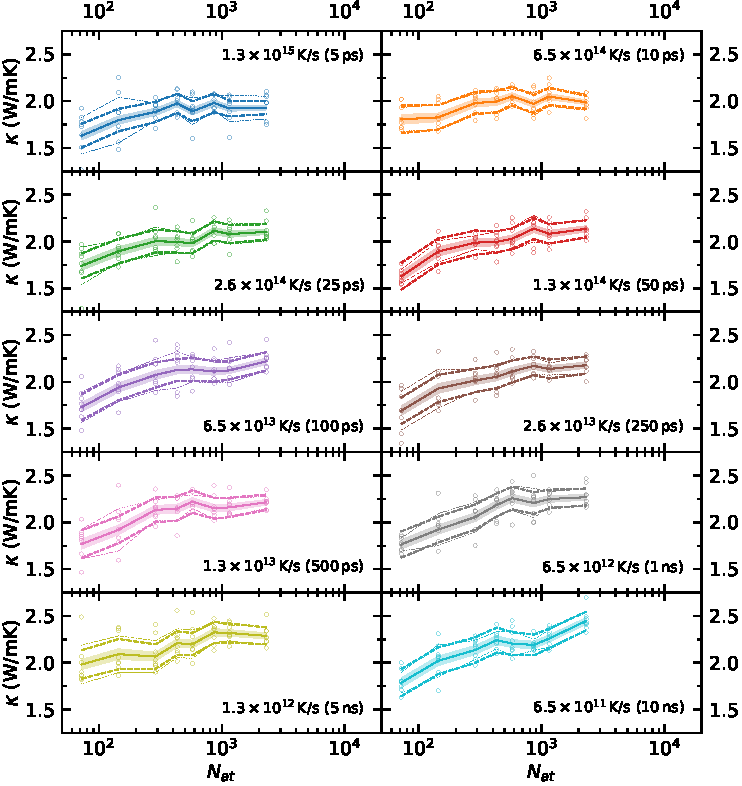
\includegraphics[width=\textwidth]{chapters/appendix/figures/Silica_NPT_kappa_NATconv.pdf}
    \caption{Thermal conductivity of a-SiO$_2$ at $500\un{K}$ obtained by a quench in the NPT ensemble at zero-pressure and with cooling rate $\gamma$. 
    The abscissa indicate the number of atoms of the system, each panel corresponds to a different quenching rate $\gamma$ (the relative quenching time $t_\mathrm{quench}$ is indicated in brackets). 
    The same symbols as Fig.~\ref{fig:results-class-kappa-vs-size} are used.
    }
    \label{fig:appendix-silica-class-npt-kappa-vs-size}
\end{figure}

\begin{figure}[!htb]
    \centering
    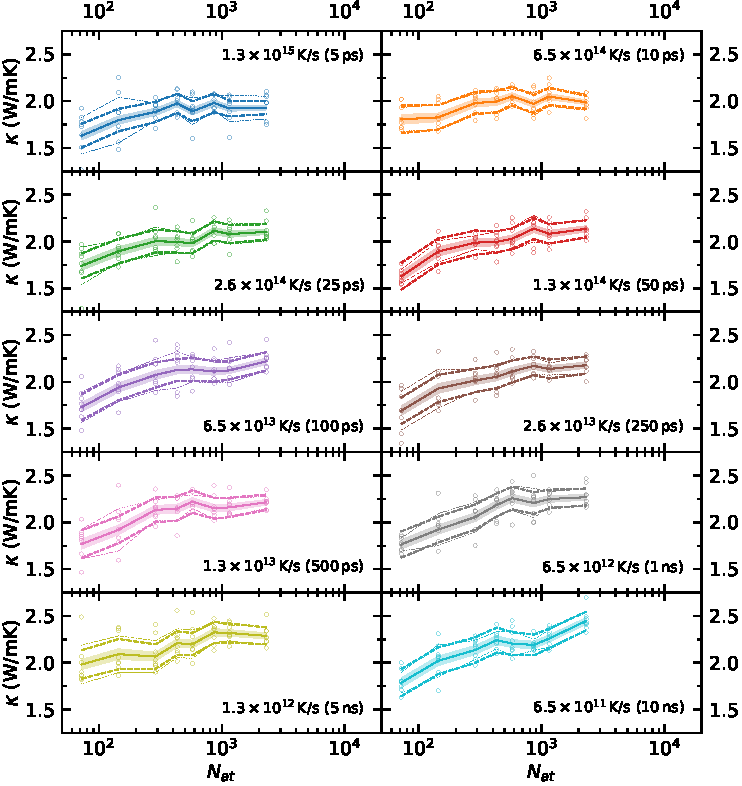
\includegraphics[width=\textwidth]{chapters/appendix/figures/Silica_NPT_kappa_NATconv.pdf}
    \caption{Thermal conductivity of a-SiO$_2$ at $500\un{K}$ obtained by a quench in the NPT ensemble at zero-pressure and with cooling rate $\gamma$. 
    Each panel corresponds to a different system size with $N_{at}$ atoms.
    The same symbols as Fig.~\ref{fig:results-class-kappa-vs-quench} are used.
    }
    \label{fig:appendix-silica-class-npt-kappa-vs-quench}
\end{figure}

\begin{figure}[!htb]
    \centering
    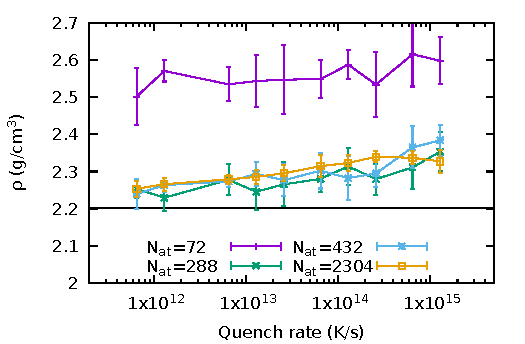
\includegraphics[width=12cm]{chapters/appendix/figures/dens_NPT_quench.pdf}
    \caption{Average density of a sample of $N_\mathrm{at}$ atoms at $500\un{K}$, obtained from a quench in the NPT ensemble at zero-pressure as a function of the quenching rate. The black line indicates the experimental value $\rho=2.202\un{g/cm^3}$. }
    \label{fig:appendix-silica-class-npt-density-vs-quench}
\end{figure}